
\section{Lessons from Biology}

A lot of robotics research is biologically inspired. There are plenty
of primitive tiny creatures in the natural world capable of
very sophisticated behaviour. It is inspiring for a robotics
researcher to know that complex tasks can be achieved with very
limited resources, and we can learn how it can be done by studying
biological systems.

Of particular interest to this thesis are the navigational skills that
many organisms posses. It is generally assumed that sophisticated
navigational behaviour can only be made possible if an organism
maintains some form of map of the environment in their brain.  A good
overview of robotics research that mimics the navigational behaviour
of biological systems is given in \cite{bio_franz00}.

It is generally a difficult problem to decipher the exact
representation an animal is using to describe the environment. There
is only so much one can recover from observing the behaviour of an
animal. We will therefore concentrate on the studies of the spatial
representation in humans.

%{\bf Humans}\\ 
Early research in spatial representation in humans
\cite{psycho_piaget56} assumed that environmental representations are
actually stored in the brain in cartographic form.  Piaget believed
that a child's intellectual development can be divided into four
discrete stages. These are more than just convenient ways of breaking
down a description of child development. He believed that each stage
represents a qualitatively different type of understanding of the
world from the previous one, and not just a quantitative increase in
knowledge of the world. Piaget proposed the following stages:

\begin{enumerate}
\item Sensorimotor Intelligence\\
   The child's thought is almost entirely perceptual and is based on 
   interactions with objects in the environment. Representation of the
   environment is relative to his own body only.

\item Preoperational Intelligence\\
   The child's thought starts getting detached from the immediate
   environment. Objects and places in the external world become
   symbols in the mind, which can then be manipulated in a fairly
   limited way. Reasoning is intuitive rather than logical, and
   knowledge is relatively unstructured.

\item Concrete Operational Intelligence\\ 
    The child is able to imagine multiple perspectives on a situation.
    He realises that a sequence of actions can be cancelled out by
    the reverse sequence, and that the same goal can be achieved by a
    number of different means.

\item Formal Operational Intelligence\\
    Thinking becomes abstract and logical, free from direct experience.


\end{enumerate}

Piaget's theory of spatial development traces the evolution of
understanding of two related concepts: projective relations and
Euclidean geometry. As the child develops through successive stages of
cognitive structure, these concepts develop in parallel, but also
become increasingly coordinated. The child develops from early stages,
where spatial thinking is tied to his own experience and images of
the environment, to one where higher-order logical properties
(e.g. the formal mathematical and geometrical properties of a
Cartesian or Euclidean coordinate system) are applied to the relative
locations of objects in space.

The rough robotic analogy of these stages would be
\begin{enumerate}

\item No map at all, reactive navigation with collision avoidance,
  odometry-based localisation.

\item Set of routes - topological maps without cycles.

\item Topological maps with cycles.

\item Global map with single reference frame. Relative locations of
  all landmarks are known with some certainty.
\end{enumerate}

Similarly to Piaget, Siegel \& White \cite{psycho_siegel75} proposed
that adults construct a cognitive representation of the physical world
at two levels. At the first level, sequences of landmarks are linked
to the route. Each landmark has directional information attached to
it: ``turn left after passing 7/11 store''. Distances are left
unspecified. As an adult gains experience of the environment, he
incorporates a sense of relative distances between landmarks. As this
information gets incorporated into the map it becomes possible to
recover bearing between any two points in the environment regardless
of whether or not they are adjacent.

Siegal \& White \cite{psycho_siegel75} see this process as the first
step in the coordination of routes into a fully metric survey-like
representation of the environment (equivalent of stage 4 in Piaget model).

However, many researchers disagree with the idea that the human brain
stores a cartographic representation of the environment. Kuipers
\cite{psycho_kuipers82} argues that such a single metric
representation would commit the system to a high degree of accuracy
and would thus not support states of partial knowledge. He argues that
a single mistake on such a representation would be very costly to
rectify at a later date, requiring the readjustment of large portions
of the representation.

Golledge \cite{psycho_golledge87} suggested that we may accurately
represent the metric relations (i.e. distance and direction) between a
limited number of major reference points, and that these then become
fixed points of reference for more local groupings at a lower
hierarchical level. We thus locate one of the minor landmarks by first
orienting ourselves towards its nearest major reference landmark; from
this we can then infer the route to the minor landmark. The relative
orientations of the fixed systems are poorly specified and retain some
subjective component; thus it is problematic to infer relative
location directly between minor points in different systems. One must
rather go up and down in the hierarchy.

I personally tend to agree more with Golledge's point of view. For
instance I can easily point in the direction of the coffee machine
when I am in my office at university, in addition, I can tell how it
is oriented relative to my desk.  However I can provide only a rough
estimate of the direction to my house, and a rather poor distance
estimate, and I am really uncertain about the orientation of my house
relative to the coffee machine in the university. 

%\SILENT{need a summary on the observation that local things are
%  metric, but further things are topological.}

%Other interesting references: 
\nocite{psycho_tversky81}
\nocite{psycho_mcnamara86} 
\nocite{psycho_passini84}
\nocite{psycho_piaget60}

\section{Robotic Mapping}

\SILENT{Introduce metric/topological mapping. Introduce EKF, FastSLAM,
  EM. State how topological and metric were rather disjoint. Maybe
  borrow some text from the next section. Future reference to the next
  chapter that defines EKF and FastSLAM in a formal way.}

There are two main paradigms of robotic mapping: topological and
metric. The topological map is essentially a graph.  Nodes of the
graph represent places in the environment. Edges of the graph
correspond to routes between places. Every edge contains some
information on how to get from one node to another. This information
can be metric (e.g. go east for about 10m), but is generally too
coarse, sufficient only to get a robot moving in the right direction.
The robot is expected to rely on its path following (go down the
corridor, for example) and place recognition skills for navigation. An
example of a topological map used by people is a subway schematic (See
\refFigure{fig:subway}).

\begin{figure}[h]
\begin{center}
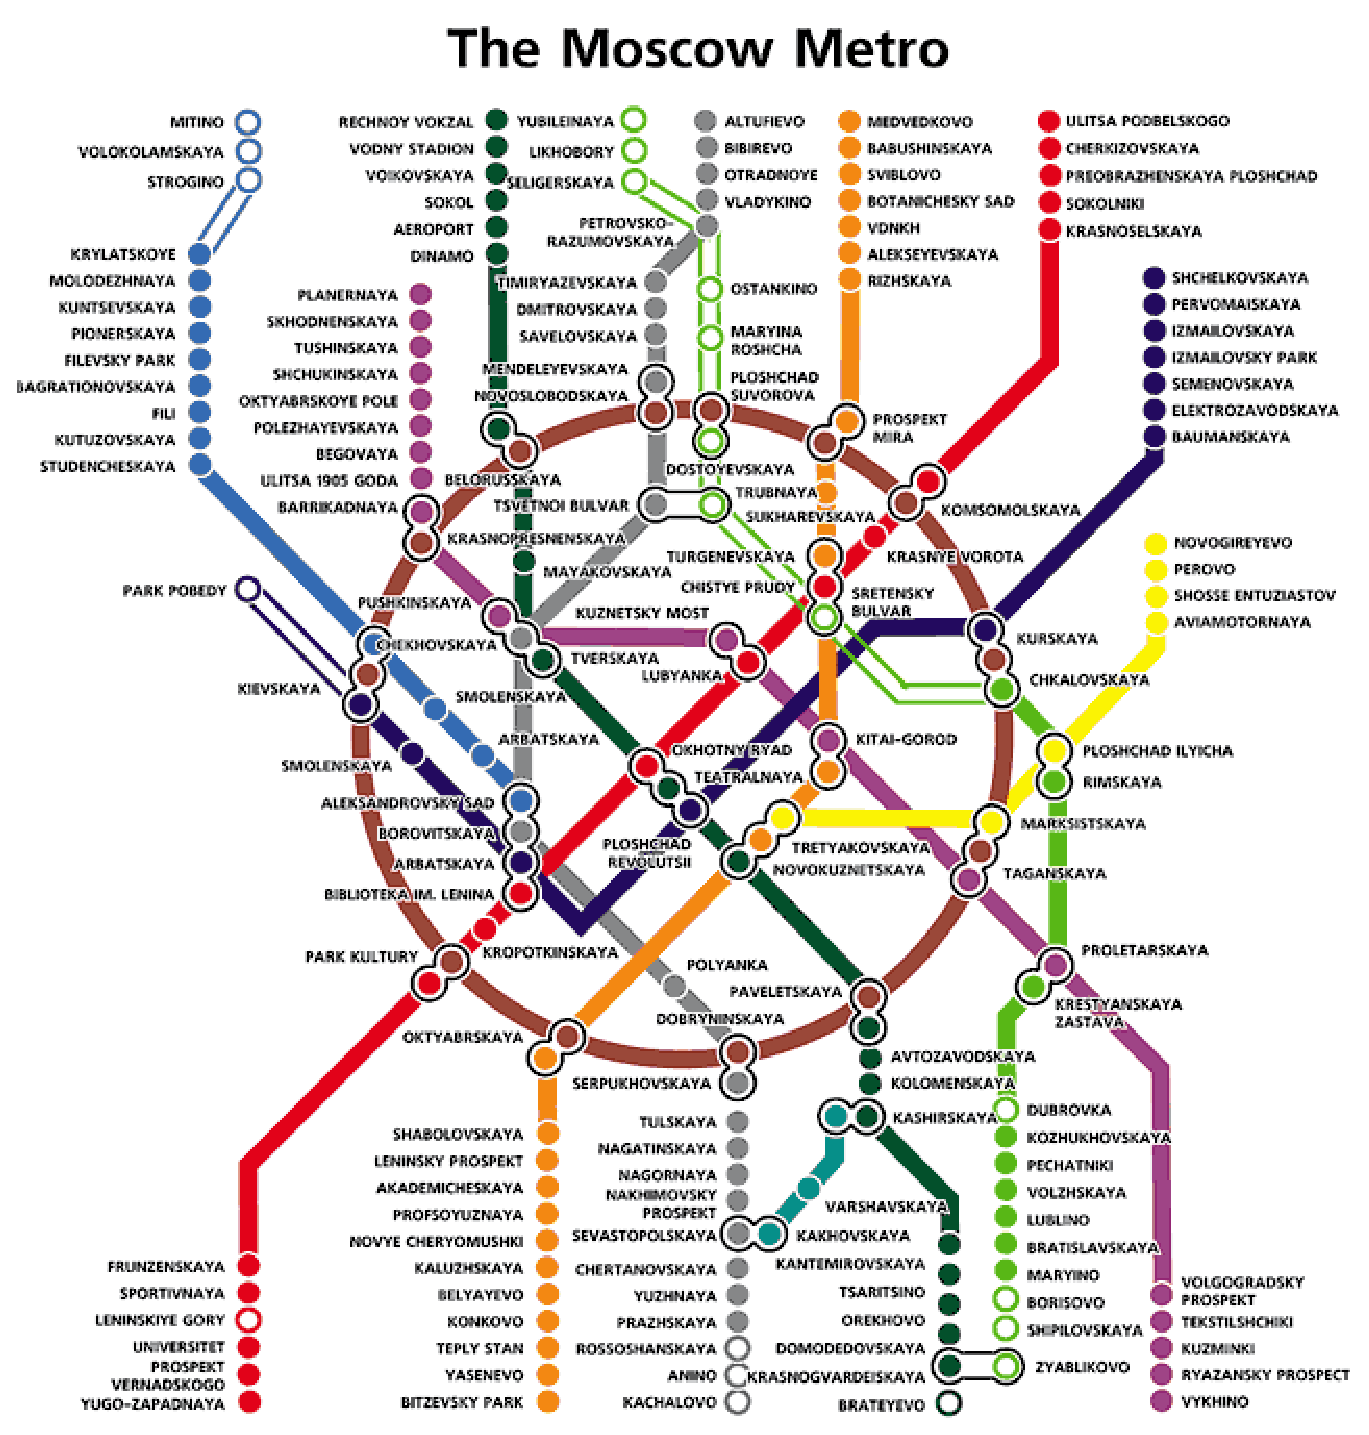
\includegraphics[width=8cm]{Pics/subway_map}
\end{center}
\caption{An example of a topological map, the Moscow subway map.}
\label{fig:subway}
\end{figure}

With a topological map, the robot is restricted to the routes along
the edges of the map. The robot cannot take shortcuts even if they are
physically possible. 

%\NOTE{cite topological papers}

Metric maps are generally more detailed and hence useful. 
The robot pose and the map features are defined in a single
reference frame. Metric maps can have landmarks (unique or identical),
or they can represent the environment as an occupancy grid. Each cell
of an occupancy grid map is assigned a probability value of being
``occupied by an obstacle''. A hybrid metric map, that combines
landmarks and occupancy grids has also been proposed in
\cite{guivant03}.  

The most common approach to Simultaneous Localisation and Mapping
(SLAM) is based on Extended Kalman Filter
\cite{ekf_slam,dissanayake01}. A more recent development is FastSLAM
\cite{fastslam,nieto2003} and a continuation of this work
FastSLAM 2.0 \cite{fastslam2}.



\section{Limitations of Metric Approaches to Mapping}

%Until recently there were two main strategies for map representations
%in robotics: topological and metric. 
%Problems with global mapping.
%Building an accurate metric map is not a trivial matter. 

There exist several good methods for building metric maps, but they do
not scale up to big environments. The main restricting factors are:

\begin{enumerate}
 \item Increase in the computational complexity. The larger the
  environment the longer it takes to execute an update with every new
  measurement.

 \item Increase of the robot pose uncertainty. As you run the
 algorithm for longer, errors tend to accumulate, especially in large
 environments. No matter how accurate your mapping process is,
 there is still going to be some residual uncertainty, and it will
 accumulate as the robot travels longer distance. The effect of such approximation
 errors is especially harmful when cycles are present.

 \item Increasing approximation error in the mapping procedure.

\end{enumerate}

The first point is fairly obvious: more landmarks require more
computation and more memory. Since the environment is considered as a
whole, one needs access to all landmarks to continue mapping. This
problem was tackled by Williams \etal\ using Constrained Local Submap
Filters \cite{williams:acra2001}. Their approach uses local maps for
building the immediate environment around the robot, effectively
forgetting about the rest of the world. The local map is then merged
into the global reference frame. This keeps the computational
requirements relatively constant, irrespective of the environment
size. The underlying mapping algorithm used in this approach is EKF
SLAM.

Increasing uncertainty is another fundamental problem, when a map is
built incrementally, i.e. new measurements are added to the existing
map as they arrive. In order to add a measurement the robot needs to
solve a data association problem: is this observation from one of the
features already in the map, is it new or is it noise?  As the robot's
pose uncertainty in the existing map increases, data association
becomes more difficult. An incorrect data association decision becomes
more likely, leading to inconsistent maps. Even in the case when
perfect data association is possible (when unique landmarks are used),
increasing pose uncertainty will cause problems, since pose
uncertainty also means map uncertainty. Even if the robot manages to
re-localise itself, correcting the map can be a problem.

The problem of data association under uncertainty has been addressed
by \cite{neira01:_data_assoc_stoch_mappin_using,
  tardos02:_mappin_local_indoor_envir_using_sonar_data}.  Rather than
finding the mapping of a single observation to a landmark, these
approaches consider a set of observations simultaneously. While such
approaches make data association more robust to sensor pose
uncertainty, they do not completely resolve the problem of {\it
  increasing} uncertainty.


Algorithms that work on all of the data at once, like Expectation
Maximisation \cite{thrun98:_probab}, are not affected by this problem,
but their computational requirements are huge and they cannot operate
in real time, since all of the data has to be processed at once.

In the case of FastSLAM, data association is solved on a per particle
basis. Data association is therefore not affected by the increasing
uncertainty. FastSLAM can also correct the map after loop closing
automatically and in real time, by simply keeping only the ``good''
particles. Nevertheless the increasing uncertainty is still a
problem. In order to perform reliably, FastSLAM will require more and
more particles to accurately represent the increasing robot pose
uncertainty. Like any particle filtering algorithm, FastSLAM is
affected by the particle depletion problem: if there are not enough
particles in the right region, the algorithm will fail to detect a
loop-closing.

EKF SLAM tends to underestimate robot pose uncertainty, and as a
result it might fail to detect loop closing. Correcting the map and
the path, even if the robot does re-localise itself, is also a big
problem for EKF SLAM, and does require substantial computational
resources.

Another important limitation comes from the approximation error. Every
mapping algorithm is trying to compute the map as a joint posterior
distribution of robot poses and a map given all the observations and
control inputs. Formal definition of the problem is given in the next
chapter.

%\begin{equation}
%\nonumber
%p(\Xall{k}{}{}, \map{k}{}{} | \Zall{k}{}, \Uall{k}{},\x{0}{}{}).
%\end{equation}

Since computing such a distribution in its true form is rather
impractical, all existing approaches try to approximate it. EKF SLAM
linearises the motion and observation models. FastSLAM approximates
the robot pose by the set of particles, and assumes a Gaussian
observation model. EM based SLAM has to make some assumptions about
the environment and the robot motion. As the environment size
increases the effect of approximation becomes more significant.



\subsection{Divide and Conquer} 

If one segments the environment into a number of smaller regions, and
maps each region separately (build local maps), one can avoid the
problem of unbounded complexity and also reduce the effects of
approximation errors.

Hybrid topological/metric maps
\cite{fergusson2003,bosse02atlas,Thrun98a} allow for accurate local
positioning by virtue of the metric component, yet are easier to
construct since computational complexity per local map is bounded. It
is also easier to close large cycles since closing a cycle in such a
map is just a matter of adding a link between two places in the
topological structure of the map.

Existing hybrid approaches can be grouped into three broad
categories: mainly metric, mainly topological, and truly hybrid. They
are all hybrid, they all use both metric and topological
representations, but some are more hybrid than others.

Mainly metric approaches desire to build a global metric map
\cite{Thrun98a, slam_thrun98b}. These approaches use topological
structure as an intermediate step only. The environment is split into
local maps, each local map is explored separately, and all maps are
then merged into a large, global map. Merging can happen incrementally
or as a single post-processing step. Some optimisation steps might be
used to enforce consistency of the global map. The main advantage of
such methods is a more robust loop closing behaviour. This is due to
the fact that loop closing is performed based on map matching.

Approaches that are more topological than metric build a topological
map \cite{Cho01,Kuipers00}. Metric maps are built for every node of
the topological map as an after thought. The relationships between
nodes is purely topological. Metric information is only used inside
the local maps.

The approaches that I consider ``more hybrid'' include \Atlas\ by
Bosse \etal\ \cite{bosse02atlas} and the one described in this thesis.
These approaches incorporate metric information into the topological
structure of the map. Every link in the topological structure stores
the spatial relation between the two nodes (local maps) as a
stochastic variable. In the case of \Atlas\ spatial relationships are
approximated by a Gaussian. There is no single global reference
frame, but it is possible to compute the relative poses of any two
local maps with some certainty, hence it is possible to project the
robot pose estimate from one reference frame to any other, along with
the uncertainty.

\Atlas\ is capable of mapping large cyclic environments. When closing
large cycles, this approach relies on place recognition (map matching)
and a robot pose estimate to detect a revisiting event. If the two
maps match, and the robot pose derived from the match is likely, a new
link can be added to the topological structure. In order to avoid
false positives, a loop closing hypothesis is first tested by
considering how well the observations match the map.


\nocite{tim_bailey,
thrun00,
dissanayake01,
SOG-Slam01,
guivant02:_simul,
guivant02:_solvin,
thrun02:_robot_mappin,
 zunino01:_simul,
 JensfeltKristensen01,
 JensfeltWijkAustin00a,
 JensfeltAustinWijk00b,
 anguelov02,
 hahnel02:_map,
 burgard99:_exper,
 schulz01:_track_multip_movin_objec_mobil_robot,
 castellanos99:_spmap,
 castellanos01:_multis,
 dudek00:_robus_place_recog_local_appear_method,
 konolige99:_increm_mappin_large_cyclic_envir,
 lu97:_global,
 gutmann96:_amos,
 williams:icra2002,
 williams:acra2001,
 Zimmer96,
 slam_kuiper91,
 slam_kuipers88,
 Thrun00j,
 Fox99,
 Cox91,
 Borenstein96,
 kk2002,
 sidenbladh00stochastic,
 Cox94,
 Thrun02h,
 Bennewitz02a,
 Liu01a,
 Dellaert00c,
 nieto2003, 
 konolige99,
 doucetraoblackwellised,
 guivant03,
 newman03,
 vandermerwe00_tr,
 vandermerwe2000,
 wan01unscented,
 unscented,
 Margaret_hybrid_maps,
 kuipers1978,
 KuipersLevitt88,
 Kuipers00,
 Buzan04,
 uhlmann97nondivergent,
 julier97new,
 julier96general,
 julier99scaled,
 doucet98sequential,
 DA_Lazy,
 Kuipers2004,
 kk2004}



% LocalWords:  Sensorimotor Preoperational odometry EKF FastSLAM Kalman
